\def\year{2018}\relax
%File: formatting-instruction.tex
\documentclass[letterpaper]{article} %DO NOT CHANGE THIS
\usepackage{aaai18}  %Required
\usepackage{times}  %Required
\usepackage{helvet}  %Required
\usepackage{courier}  %Required
\usepackage{url}  %Required
\usepackage{graphicx}  %Required
\usepackage{amssymb}

\usepackage{algorithm}
\usepackage[noend]{algpseudocode}
\usepackage{multirow}

\usepackage{amsmath}
\usepackage{amssymb}
\usepackage{bm}
\usepackage{balance}



\frenchspacing  %Required
\setlength{\pdfpagewidth}{8.5in}  %Required
\setlength{\pdfpageheight}{11in}  %Required
%PDF Info Is Required:
\pdfinfo{
	%/Title (Improving Coherence of Neural Extractive Summarization with Reinforcement Learning)
	/Title (Learning to Extract Coherent Summary via Deep Reinforcement Learning)
	
	/Author (Yuxiang Wu, Baotian Hu, Qiang Yang)}
\setcounter{secnumdepth}{0}  
\begin{document}
	% The file aaai.sty is the style file for AAAI Press 
	% proceedings, working notes, and technical reports.
	%
	\title{Learning to Extract Coherent Summary via Deep Reinforcement Learning}
	\author{Anonymous authors}
	\maketitle
	\begin{abstract}
		 Coherence plays a critical role in producing high-quality summary from a document. In recent years, neural extractive summarization is becoming increasingly attractive. However, most of them ignore the coherence of summary when extracting sentences. As an effort towards extracting coherent summaries, we propose a neural coherence model to capture the cross-sentence semantic and syntactic coherence patterns. The proposed neural coherence model obviated the need for feature engineering and can be trained from scratch in an end-to-end fashion using a large corpus. Empirical results show that the proposed neural coherence model can effectively capture the cross-sentence coherence patterns. Using the output of the neural coherence model and ROUGE as the reward, we design a reinforcement learning method to train the neural extractive summarizer. The extractive model learns to optimize coherence and informative importance of the summary simultaneously. Experiment result shows that the proposed approach outperforms existing baselines and achieves the state-of-art performance in terms of ROUGE on CNN/Daily Mail dataset. The qualitative evaluation indicates that the summary produced by the proposed approach is more coherent and readable.
	\end{abstract}
	
	
	\section{Introduction}
	Although deep learning has dominated almost every field of natural language processing, such as sentiment classification\cite{duyutang-sentiment}, machine translation\cite{cho-translation}, generating high-quality summaries from long documents is still a very challenging task. Most of the recent works on abstractive summarization focus on headline generation from one paragraph~\cite{fb2015} or several sentences~\cite{lcsts} by using sequence-to-sequence architectures borrowed from neural machine translation. However, all of them bypass the fundamental problems of abstractive summarization, namely the representation of long documents and consecutive sentences generation. These models can not generate readable, informative and coherent sentences when dealing with full documents.  There is still a long way for abstractive summarization to be practicable.
	
	In contrast, extracting sentences from document to form summary, also named extractive summarization, is a more practical way, because it can guarantee the grammatical correctness and semantic relevance with the document of the produced summary. Extractive summarization has been researched for several decades. Traditional approaches mainly focus on scoring sentences of the document by using a graph-based method or integer linear programming, coupling with human-engineered features. As the distributed representation shows its outstanding performance to capture the semantic and syntactic information of text~\cite{word2vec,nc_baotian}, there is an emergence of works that use the deep neural network to extract salient sentences~\cite{SummaRuNNer,nayeem2017extract,jianpeng2016}. Although both of traditional methods and deep neural network based methods can identify the important sentences of the documents, both of them lead to the problem in overall coherence of the summary. Sometimes there are several topics in the summary and the interpretation of one sentence do not depend on its neighbors, which causes that the summary can not express a meaning as a whole. 
	
	The coherence of summary is essential for its readability and clarity. In the past decades, research works mainly focus on topical coherence. The most popular method is the entity grid model\cite{entitygrid} which constructs a grid to represent grammatical and semantic transitions of entities between sentences. The entity grid is then converted to discrete feature vectors which are used as input to learning model to obtain the coherence score of the texts\cite{nlcm}. The entity grid model needs the entity labels of words in sentences. The performance of name entity recognition algorithm may become the bottleneck of the grid model. The entity grid model uses a discrete representation of text, which can not model long entity transitions. In this paper, we propose neural coherence model which can learn the coherence degree of two sentences with the distributed representation of text in an end-to-end fashion.
	
	
	Due to the avoidance of lots of handcrafted features, the neural extractive summarization is becoming increasingly popular.  The core contribution of most of these works is using the deep neural network to obtain the distributed representation of documents and sentences, to extract informatively important sentences\cite{jianpeng2016}. To our knowledge, there is no work incorporating the coherence into the neural extractive model while extracting sentences. It is difficult to incorporate coherence into optimization objective of supervised learning because coherence also depends on sentences that are eventually extracted when inference is performed. Reinforcement learning (RL) aims to train an agent to obtain the maximum reward when it interacts with a given environment. RL is usually used in the case that the evaluation metrics to be optimized is not differentiable and traditional supervised learning methods cannot be used. RL has been used in sequence generation tasks such as abstractive summarization generation~\cite{socher2017_summarization} and neural machine translation by optimizing the metrics such as BLEU, ROUGE or METEOR~\cite{rl2nmt}.
	
	In this paper, we focus on improving the coherence ability of neural extractive model via reinforcement learning. Our first contribution is to propose a novel neural coherence model which uses the low-dimension dense distributed representation of texts instead of sparse discrete features. The proposed neural coherence model does not rely on any entity recognition systems and can be trained almost from scratch in an end-to-end fashion. The neural coherence model can capture the cross-sentence local entity transition and discourse relation with the layer by layer convolution and max-pooling layers. It is feasible to train the neural coherence model with large scale unlabeled plain text. The experiment results show that, give one sentence, the neural coherence model can identify the appropriate next sentence to compose a coherent sentence pair effectively. 
	
	
	Our second contribution is the reinforcement learning solution for training neural extractive summarization model. Although reinforcement learning has been applied to abstractive headline generation with Rouge or BLEU metrics as rewards\cite{socher2017_summarization,ayana2016}, to our knowledge, we are the first to design the reinforcement learning to neural extractive model with the neural coherence and rouge score as the reward. After training with our proposed approach, the neural extractive model can balance between the coherence and informative importance of sentences effectively. We experimentally evaluate our approach on standard task and show that it can achieve state of the art performance on rouge metrics. The qualitative evaluation indicates that the summary produced by our system are more informative and coherent.
	
	
	\section{Related Work}
	Our research is build on previous works in the field of neural extractive summarization, reinforcement learning and coherence models.
	
	Much progress has been made beyond traditional frameworks of extractive summarization models. Most of recent works are based on deep neural networks and distributed representation of text, which regards the extractive summarization as sentence sequence labeling problem. For example, \cite{jianpeng2016} use convolutional neural network to encode sentence, and then recurrent neural network takes in the sentence representation sequentially to encode the document. Finally they use another recurrent neural network to label sentences sequentially, taking the encoded document representation and the previously labeled sentences into account. \cite{jianpeng2016} mainly consider the importance of the sentence and the non-redundancy of the summary. \cite{SummaRuNNer} use the similar architecture to encode document, but add the information content, salience and novelty into the model when labeling sentences. The model proposed by \cite{SummaRuNNer} is very interpretable, since it allows visualization of its predictions. 
	
	Our work is also related to the application of reinforcement learning on document summarization. Different from text classification whose target is the clear single or multiple labels, the targets of machine translation or automatic text summarization are many potential sequence of words, which own its property independent of input. Such tasks are natural candidate problems for reinforcement learning by using some evaluation metrics to judge the quality of the result such as BLEU, ROUGE and et al. Deep reinforcement learning has drawn great attention in recent years. For example, \cite{socher2017_summarization} use the ROUGE-L score as a reinforcement reward and self-critical policy gradient training algorithm to train a abstractive summarization models. \cite{ayana2016} and \cite{sltrnn2016} show optimizing the evaluation metrics ROUGE directly via reinforcement learning is more effective than optimizing likelihood for the decoder generation. All of above works focus on abstractive summarization by optimizing ROUGE metrics, To date, there are no work to apply RL with coherence as reward to neural extractive summarization. To our knowledge, our work is the first step toward this goal.
	
	
	A key requirement for summarization systems is the coherence of its output. Coherence is which makes multiple sentences semantically, logically and syntactically coherent\cite{Yao2017RecentAI}. Not surprisingly, a variety of coherence methods have been developed over the years\cite{Yao2017RecentAI}, among which entity grid models is the most popular one proposed by\cite{entitygrid}. However, the discrete representation of entity grid suffer from the severe curse of dimensionality problem which limit the its application on text summarization. \cite{nlcm} presented a local coherence model based on a convolutional neural network that operates over the distributed representation of entity grid. However \cite{nlcm} still rely on the name entity tools to identify the name entity of sentences first. \cite{jiweili2014}  use the recurrent or recursive neural network to obtain the distributed representation of sentences and then use pairwise ranking method to train the coherence model. \cite{jiweili2014} select the window of sentences from original articles as positive examples, and random replacement of some sentences in the window as negatives examples. This model does not need any feature engineering, but this model is hard to capture the local entity transition for lack of cross-sentence local interaction. Our neural coherence model can be trained almost from scratch in an end-to-end fashion. It can also model the local entity transition and syntactical relation between sentences via different level cross-sentence local interaction. 

	\section{Neural Sentence Extractor}
	
	The prerequisite of using proposed reinforcement learning approach is to construct an neural extractive summarization model. In this work, we use the state of the art extractive summarization model similar to SummaRuNNer proposed by\cite{SummaRuNNer}. The extractive summarization model reads the document and selects a set of sentences sequentially as summary.  
	
	Given a document $X=(x_1, x_2, \cdots, x_n)$ that has $n$ sentences, the neural extractive summarization models aim to generate a sequence of binary decisions $Y=(y_1, y_2, \cdots, y_n)$, where $n$ the number of sentences in the document and $y_i \in \{0,1\}$ indicates whether sentence $x_i$ is selected. The $i$-th sentence is selected as part of summary if $y_i=1$, and ignored otherwise.
	
	
	We use a hierarchical neural network to model the document. At the word-level, CNN is used to extract features of words and their context. Let $x=(w_1, w_2, \cdots, w_m)$ denotes a sentence with $m$ words, and $l$ denotes the size of word embedding. Then the sentence could be represented by a matrix $\mathbf{M} \in \mathbb{R}^{m \times l}$. Multiple convolution kernels with different kernel size are used to extract features
	$$\mathbf{f}_i^j = \mathbf{M}_{i:i+k_j-1} \odot \mathbf{W}_j + b_j ,$$
	where $\odot$ represents element-wise product, $\mathbf{W}_j, k_j, b_j$ denote the kernel weight matrix, kernel size and bias of the $j$-th convolution kernel respectively. The word $w_i$ is represented by concatenating the feature maps $\mathbf{f}_{w_i}=[\mathbf{f}_i^1 ; \mathbf{f}_i^2 ; \cdots]$. The representation of sentence $x$ is represented by the mean of all its word features:
	$$ \mathbf{x} = \frac{1}{m} \sum_{i=1}^m \mathbf{f}_{w_i} .$$
	
	At the sentence-level, we use a bi-directional gated recurrent unit (Bi-GRU) to model the context of sentences. Gated recurrent unit is a variant of recurrent neural network proposed by \cite{chung2014empirical}. It has two gates, an update gate $\mathbf{z}_t$ and reset gate $\mathbf{r}_t$. The hidden state $\mathbf{h}_t$ at time step $t$ could be computed with following equations:
	\[ \mathbf{z}_t = \sigma(\mathbf{W}_{z} \mathbf{x}_t + \mathbf{V}_{z} \mathbf{h}_{t-1}  + \mathbf{b}_{z}) , \]
	\[ \mathbf{r}_t = \sigma(\mathbf{W}_{r} \mathbf{x}_t + \mathbf{V}_{r} \mathbf{h}_{t-1}  + \mathbf{b}_{r}) , \]
	\[ \hat{\mathbf{h}}_t = \tanh(\mathbf{W}_{h} \mathbf{x}_t + \mathbf{V}_{h} (\mathbf{r}_{t} \odot \mathbf{h}_{t-1} ) + \mathbf{b}_{h} ) ,\]
	\[ \mathbf{h}_t = (1 - \mathbf{z}_t) \odot \hat{\mathbf{h}}_{t} +  \mathbf{z}_t \odot \mathbf{h}_{t-1} ,\]
	where $\mathbf{W}$'s, $\mathbf{V}$'s and $\mathbf{b}$'s are trainable parameters of GRU. 
	
	Using Bi-GRU, the representation of the $t$-th sentence $\mathbf{x}_t$ is transformed to a forward hidden state $\overrightarrow{\mathbf{h}}_t$ and a backward hidden state $\overleftarrow{\mathbf{h}}_t$. Both states are are concatenated to form the contextual representation of $t$-th sentence $\overleftrightarrow{\mathbf{h}}_t = [\overrightarrow{\mathbf{h}}_t ; \overleftarrow{\mathbf{h}}_t]$. The entire document is represented by a non-linear transformation of of the mean-pooled $\overleftrightarrow{\mathbf{h}}_t$'s:
	\[ \mathbf{d} = \tanh( \mathbf{W}_d (\frac{1}{n} \sum_{t=1}^{n} \overleftrightarrow{\mathbf{h}}_t ) + \mathbf{b}_d ) ,\]
	where $\mathbf{W}_d$ and $\mathbf{b}_d$ are parameters of the transformation, and $n$ is the number of sentences in the document. 
	
	The probability of extraction decisions $Y$ conditioned on document $X$ could be factorized as $\Pr(Y|X) = \prod_{t=1}^{n} \Pr(y_t | X, y_{1:t-1})$.
	The probability of extracting the $t$-th sentence is given by the following equation:
	\begin{equation} \label{eq:mlp}
		 \Pr(y_t=1|X, y_{1:t-1}) = \text{MLP}(\overleftrightarrow{\mathbf{h}}_t, \mathbf{g}_{t-1}, \mathbf{d}, \mathbf{e}_t^{abs}, \mathbf{e}_t^{rel} ) ,
	\end{equation}
	where $\text{MLP}(\cdot)$ means a multilayer perceptron that outputs a probability, $\mathbf{g}_t$ represents all sentences selected in history, $\mathbf{e}_t^{abs}$ and $\mathbf{e}_t^{rel}$ are absolute and relative position embeddings respectively. In supervised learning setting, the history selections are calculated by
	\begin{equation}
	\mathbf{g}_t = \mathbf{g}_{t-1} + \dot{y}_t \overleftrightarrow{\mathbf{h}}_t ,
	\end{equation}
	where $\dot{y}_t$ is the ground truth selection label. In reinforcement learning setting, $\dot{y}_t$ is replaced with the selection action $\tilde{y}_t \sim \Pr(y_t=1|X) $ sampled with the estimated selection probability. Details of reinforcement learning will be introduced later.
	
	\textbf{TODO} Trained with cross-entropy loss.
	
	\section{Extract Coherent Summary with Reinforcement Learning} 
	\subsection{Reinforcement Learning}
	The problem of extractive summarization could be formulated as a reinforcement learning problem. The neural sentence extractor can be considered as an \emph{agent} that extracts sentences sequentially from documents. At each time step $t$, the agent is in \emph{state} $s_t = (X, y_{1:t-1})$ which includes the document and previous selections. Agent would take a \emph{action} $y_t \in \{0,1\}$ that decides whether sentence $x_t$ is extracted or not. After the agent takes the action $y_t$, it may receive an immediate reward $r_{t}$ that shows how good the action is. The reward could be delayed. When the agent finishes extracting sentences from the whole document, it also receives an final reward $r_{-1}$ that indicates performance of the entire action sequence $(y_1, y_2, \cdots, y_n)$.
	
	We use the REINFORCE algorithm to train our neural sentence extractor. It is a kind of policy gradient method proposed by \cite{williams_simple_1992}, and it maximizes agent's performance by updating its policy. The policy is defined as the probability of taking an action at time $t$ given the state, which is parameterized by $\Theta$:
	\begin{align}
	\pi(a|s_t,\Theta) &\triangleq \Pr(y_t=a|s_t,\Theta) \\
	&\triangleq \Pr(y_t=a|X, y_{1:t-1}, \Theta) .
	\end{align}
	In this case, $\Theta$ represents all the parameters in the neural sentence extractor. We use a shorthand $\pi_{\Theta}$ to denote the policy $\pi$ parameterized by $\Theta$. By applying Equation \ref{eq:mlp}, we have:
	\begin{equation}
	\pi_{\Theta}(a=1|s_t) = \text{MLP}_{\Theta}(\overleftrightarrow{\mathbf{h}}_t, \mathbf{g}_{t-1}, \mathbf{d}, \mathbf{e}_t^{abs}, \mathbf{e}_t^{rel} ) ,
	\end{equation}
	
	Let $s_0=X$ represents the initial state when no actions are taken yet, and $v_{\pi_{\Theta}}(s)$ be the \emph{value} function that represents the expected \emph{return} starting with state $s$ by following policy $\pi_{\Theta}$. Return at time $t$ is defined as $R_t=\sum_{i=t}^{\infty} \gamma^{i-t} r_i$, where $\gamma$ is the discount factor. The objective of REINFORCE is defined as maximizing the value of initial state $v_{\pi_{\Theta}}(s_0)$, or minimizing the loss $L_{RF}(\Theta) = - v_{\pi_{\Theta}}(s_0)$. Therefore, the parameters should be updated by the gradient of $L_{RF}(\Theta)$ with respect to parameters $\Theta$:
	\begin{align}
	\nabla L_{RF}(\Theta) &= - \nabla v_{\pi_{\Theta}}(s_0) \label{eq:L_RF} \\ 
	&=- \sum_{t=1}^{n} \gamma^t \Pr(s_t | s_0, \pi_{\Theta}) \sum_{a} q_{\pi_{\Theta}}(s_t,a) \nabla \pi_{\Theta}(a|s_t) ,
	\end{align} 
	where $q_{\pi_{\Theta}}(s,a)$ is the \emph{action-value} function that represents the expected return after taking action $a$ at state $s$ with policy $\pi_{\Theta}$. 
	%TODO: may give a proof of this equation in the appendix
	
	Since the state space is too large, it is infeasible to compute the exact value of the gradient. We use Monte Carlo sampling to approximate the gradient:
	\begin{align}
	\nabla L_{RF}(\Theta) &= - \mathbb{E}_{\tilde{s}_t \sim \pi_{\Theta}} \Big[ \gamma^t \sum_{a} q_{\pi_{\Theta}}(\tilde{s}_t,a) \nabla \pi_{\Theta}(a|\tilde{s}_t) \Big] \\
	&= - \mathbb{E}_{\tilde{y}_t, \tilde{s}_t \sim \pi_{\Theta}} \Big[ \gamma^t q_{\pi_{\Theta}}(\tilde{s}_t,\tilde{y}_t) \frac{\nabla \pi_{\Theta}(\tilde{y}_t|\tilde{s}_t)}{\pi_{\Theta}(\tilde{y}_t|\tilde{s}_t)}  \Big] \\
	&= - \mathbb{E}_{\tilde{y}_t, \tilde{s}_t \sim \pi_{\Theta}} \Big[ \gamma^t q_{\pi_{\Theta}}(\tilde{s}_t,\tilde{y}_t) \nabla \log \pi_{\Theta}(\tilde{y}_t|\tilde{s}_t) \Big] \\
	&= - \mathbb{E}_{\tilde{y}_t, \tilde{s}_t \sim \pi_{\Theta}} \Big[ \gamma^t \tilde{R}_t \nabla \log \pi_{\Theta}(\tilde{y}_t|\tilde{s}_t) \Big] ,
	\end{align}
	where $\tilde{s}_t$ and $\tilde{y}_t$ are randomly sampled from $\pi_{\Theta}$, $\tilde{R}_t$ is the actual return received since $\tilde{s}_t$ and $\tilde{y}_t$. Then parameters $\Theta$ is updated as follows:
	\begin{equation} \label{eq:update}
	\Theta \leftarrow \Theta + \gamma^t \tilde{R}_t \nabla \log \pi_{\Theta}(\tilde{y}_t|\tilde{s}_t) .
	\end{equation} 
	
	The definition of reward is crucial for reinforcement learning, because it determines the optimization direction. To ensure that neural sentence extractor extracts informative and coherent summaries, the reward includes both ROUGE score and coherence score. The coherence score is exploited as immediate reward $r_t$ and ROUGE as the final reward $r_{-1}$. Therefore, the algorithm is indeed maximizing the sum of both ROUGE and coherence score:
	\begin{align}
	v_{\pi}(s_0) &\triangleq \mathbb{E}_{\pi}[R_0 |s_0] = \mathbb{E}_{\pi} [ \tilde{r}_{-1} + \sum_{t=1}^{n} \tilde{r}_t ] \\
	&= \mathbb{E}_{\pi} [ \text{ROUGE}(\tilde{Y}) + \lambda \text{Coherence}(\tilde{Y}) ] , \label{eq:reward_sum}
	\end{align}
	where $\tilde{Y} = (\tilde{y}_1, \cdots, \tilde{y}_n)$ is a sampled sequence of actions, and $\tilde{r}$ is their corresponding rewards. $\lambda$ is the coefficient that balances the two rewards. The neural coherence model for computing the coherence reward is introduced in the next subsection.
	
	
	\subsection{Neural Coherence Reward}
	We propose a neural coherence reward model which is based on convolutional neural network architecture.  The neural coherence reward model has some advantages over traditional entity grid models. On one hand, the neural coherence model compute the coherence score almost from scratch. It only need take the original sentences as input. On other hand,  The neural coherence reward model use the distributed text representation which can capture long range entity transitions. The architecture of the neural coherence reward model is shown in Figure~\ref{coherence}. The Neural Coherence reward model is build on the ARC-II proposed by ~\cite{NIPS2014_hu} for sentence matching.
	
	\begin{figure}
		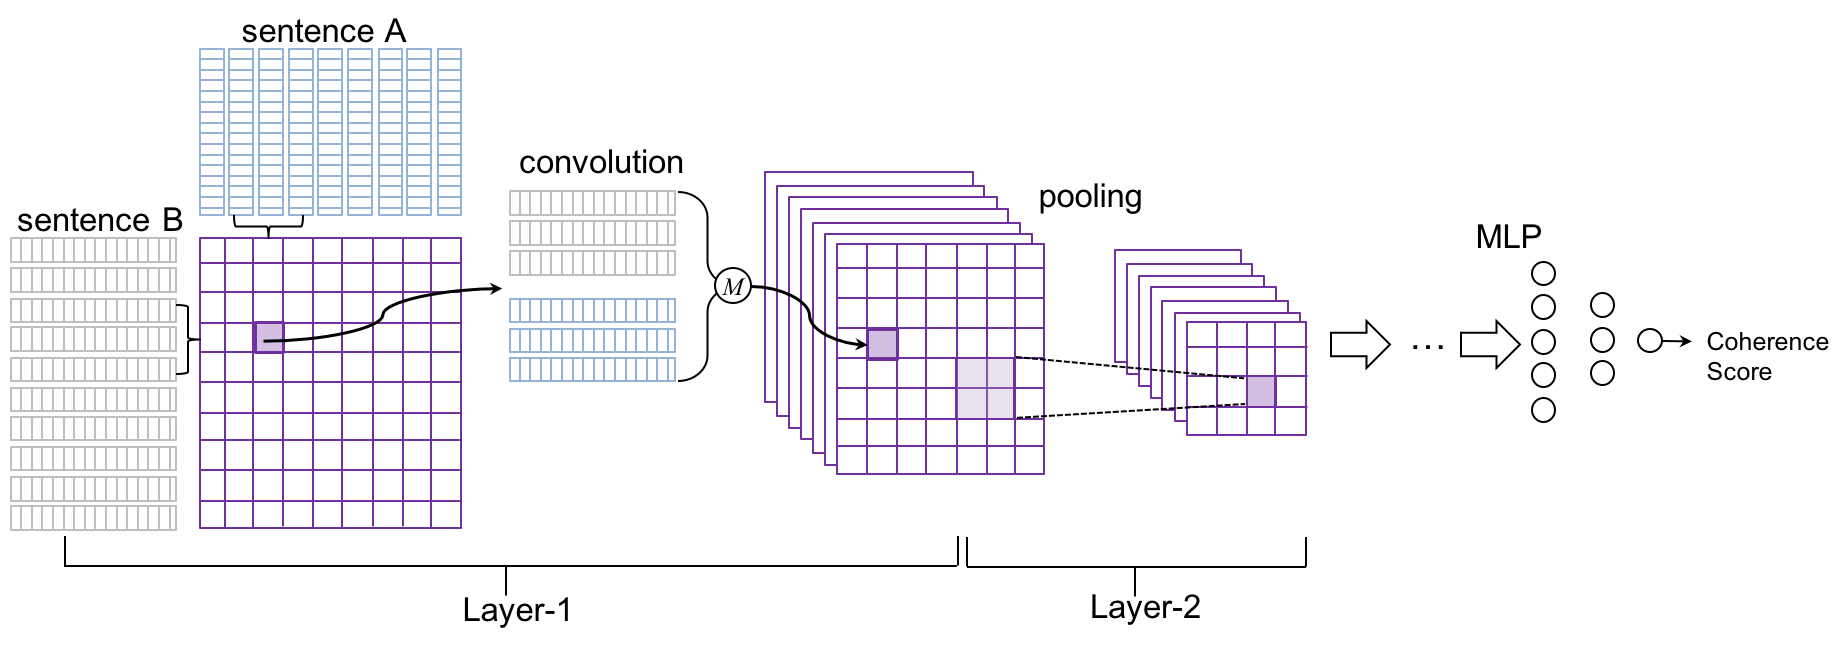
\includegraphics[width=0.5\textwidth]{./images/coherence.png}
		\label{coherence}
		\caption{Architecture of neural coherence model.}
	\end{figure}
	
	
	Given two sentences $S_X$ and $S_Y$ , the neural coherence model can model the local interaction between two sentences. In Layer-1, it takes sliding windows on both sentences to model all the possible local coherence matching of two sentences. For segment $i$ on $S_X$ and segment $j$ on $S_Y$, the local coherence matching of them is computed as Eq.~\ref{localmatching}
	
	\begin{equation}
	z^{(1)}_{i,j} \overset{\text{def}}{=}
	z^{(1)}_{i,j}(x,y) =  g(\hat{\mathbf{z}}^{(0)}_{i,j})\cdot \sigma(W^{(1)} \hat{\mathbf{z}}^{(0)}_{i,j} + b^{(1)}),
	\label{localmatching}
	\end{equation}
	
	where $W^1$ is the weight parameters for 1st layer and $b^1$ is the bias. $\sigma$ is the nonlinear function which we choose ReLU~\cite{}. $\hat{\mathbf{z}}^{(0)}_{i,j} \in \mathbb{R}^{2k_1 \times D_{e}}$ is got by concatenating the embeddings of words in $S_X$ and $S_Y$ sequentially:
	
	\begin{equation}
	\hat{\mathbf{z}}^{(0)}_{i,j} =  [e(x_i)^\top, ... , e(x_{i+k_1-1})^\top, e(y_j)^\top,..., e(y_{j+k_1-1})^\top]^\top.
	\end{equation}
	
	\noindent $g(\hat{\mathbf{z}}^{(0)}_{i,j})$ is the gate function, It equals 0 if all the element of $\hat{\mathbf{z}}^{(0)}_{i,j}$ equals 0 else 1.
	
	Layer2 takes in the output of layer-1 and performs a max-pooling in each dimension of the cells in non-overlapping $2\times 2$ windows.
	
	
	\begin{equation}
	z_{i,j}^{(2)} = \max(\{z_{2i-1,2j-1}^{(1)}, z_{2i-1,2j}^{(1)},z_{2i,2j-1}^{(1)},z_{2i,2j}^{(1)}\}). 
	\label{e:2dpool}
	\end{equation}
	
	Following Layer-2, there is more convolution and  max-pooling layers, analogous to that of convolutional architecture for image input~\cite{cnn}. Finally, we obtain the fixed length vector $h$ with dimension $m$ and feed $h$ into multi-layer perceptron (MLP), a nonlinear function $tanh$, to compute coherence score of the two sentences.
	
	\begin{equation}
	Coh(S_X,S_Y) = tanh(W  h+b). 
	\end{equation}
	
	\noindent Where  $ W \in \mathbb{R}^{1 \times m}$ is the weight parameters and $b$ is the bias. Hence, the coherence model will output a coherence score  $Coh(S_X, S_Y) \in [-1,1]$ for sentence pairs $S_X, S_Y$.
	
	
	From the first layer, the neural coherence model can learn the local interaction of $S_X$ and $S_Y$, so as to capture the local entities transition of two sentences.  And also, it can obtain higher level and wider entities transition representation of $S_X$ and $S_Y$ with more convolution and max pooling layers.
	
	
	
	For training the neural coherence model, we use a discriminative training strategy with a large margin objective. 
	Suppose we are given the following triples $(S_X, {S_Y}^{+},{S_Y}^{-})$, we have the ranking-based loss as objective:
	
	\begin{equation}
	\begin{split}
	L_\Theta({S_X}, {S_Y}^+, {S_Y}^-) = 
	\max(0, m+Coh({S_X, {S_Y}^-})\\
	-Coh({S_X}, {S_Y}^+))
	\end{split}
	\label{equation-objective}
	\end{equation}
	
	\noindent Where $0< m <1$ controlling the margin in training. In the experiments, we use $m = 1.0$. The model is trained by minimizing the above objective, to encourage the model to assign higher coherence score for coherent sentence pairs $(S_X, {S_Y}^-)$ than $({S_X}, {S_Y}^+)$. We use stochastic gradient descent (SGD) to optimize the model parameter.
	
	It is easy to construct large enough data to train neural coherence model. Given a document with sequence of $n$ sentences $S_1, S_2,...,S_n$. We can obtain the following triples $(S_l, S_{l+1}, S_j)$, where $0<l<n$. $S_j$ is randomly sampled from document and $j\notin[l,l+1]$.
	
	
	
	\subsection{ROUGE Score Reward}
	ROUGE score is also used as the final reward to ensure that the neural extractor extracts reasonably informative sentences. Given a sequence of sampled decisions $(\tilde{y}_1, \cdots, \tilde{y}_n)$, we can get the sequence of extracted sentences $G$. Since the dataset comes with summaries written by human editors, the corresponding manual summary $T$ is treated as the ground truth. Then ROUGE score $\text{ROUGE}(G, T)$ could be computed and used as a reward for the entire sampled decisions:
	\[ r_{-1}(\tilde{y}_1, \cdots, \tilde{y}_n) = \text{ROUGE}(G, T). \]
	
	The overall training algorithm is illustrated in the Algorithm \ref{algorithm-curriculum-learning}. Since REINFORCE algorithm converges very slowly, we pretrain the neural sentence extractor with supervised learning. The neural coherence model is also trained and then fixed for the coherence scoring. During the training of REINFORCE, an sequence of actions and states are sampled
	according to the policy. Then the coherence model and ROUGE are used for computing the rewards. The parameters of neural sentence extractor $\Theta$ is then updated according to Equation \ref{eq:update}. 
	
	\begin{algorithm}[t]
		\small
		\begin{algorithmic}[1]
			\State $\Psi \leftarrow$ train the neural coherence model.
			\State $\Theta \leftarrow$ pretrain the neural sentence extractor with supervised learning.

			\Loop
			
			\State $X, T \leftarrow$ sample a document-summary pair from corpus $D$
			\State $\tilde{s}_0 \leftarrow X$
			\State Sample an episode $\tilde{s}_1, \tilde{y}_1, \cdots, \tilde{s}_n, \tilde{y}_n$ following $\pi_{\Theta}$
			
			\State $previous \leftarrow \chi$ (a placeholder for empty start sentence)
			\For  {each step $t=1 \dots n$}
			\If {$\tilde{y}_t = 1$}
				\State $\tilde{r}_t \leftarrow \lambda Coh_{\Psi}(previous, x_t)$
				\State $previous \leftarrow x_t$
			\Else
				\State $\tilde{r}_t \leftarrow 0 $
			\EndIf
			\EndFor
			
			
			\State $G \leftarrow$ the sequence of extracted sentences
			\State $\tilde{r}_{-1} = \text{ROUGE}(G, T)$
			
			\For  {each step $t=1 \dots n$}
			\State $\tilde{R}_t \leftarrow \sum_{i=t}^{n} \tilde{r}_i + \tilde{r}_{-1}$
			\State $\Theta \leftarrow \Theta + \alpha \tilde{R}_t \nabla \log \pi_{\Theta}(\tilde{y}_t|\tilde{s}_t)$
			\EndFor
			
			\EndLoop
			
		\end{algorithmic}
		\caption{The overall training algorithm. $\alpha$ is the learning rate, $\chi$ is a placeholder sentence for bootstrapping the coherence score of the first extracted sentence.}
		\label{algorithm-curriculum-learning}
	\end{algorithm}
	\vspace{-4pt}

	
	\section{Experiments and Results}

	We used the CNN/Daily Mail dataset originally proposed by \cite{hermann_teaching_2015} for machine comprehension task. This dataset contains news documents and highlights crawled from CNN and Daily Mail website, and  \cite{nallapati_ramesh_abstractive_2016} propose to use it for summarization task. It is commonly used by works of extractive summarization \cite{jianpeng2016,SummaRuNNer} and abstractive summarization \cite{nallapati_ramesh_abstractive_2016,see_get_2017}. We used the scripts provided by \cite{hermann_teaching_2015} to download the dataset. It contains 287,226 documents for training, 13,368 documents for validation and 11,490 documents for test. We use the \textbf{nltk} package to segment the sentences. Since the dataset only contains manual summaries and do not have extractive labels, a greedy algorithm similar to \cite{SummaRuNNer} is used to generate extraction labels for supervised learning.
	 
	\subsection{Results of the neural coherence model}
	The coherence model is trained before applied in the REINFORCE training of sentence extractor. It uses 64-dimensional word embeddings, and the sizes of all its convolutional kernels are set to be 3. In the first layer, the 1D convolution has 128 filters. It is followed by two layers of 2D convolution, with 512 and 256 filters respectively. Each of the convolutional layers is followed by a max-pooling layer with size 2 and stride 2. The final two fully-connected layers have 512 and 256 hidden units respectively. The maximum sentence length is 50, and sentences longer than this length would be truncated. The coherence model is trained with stochastic gradient descent (SGD) with batch size 64 and learning rate 0.1. 
	
	The training triplets are sampled from the CNN/Daily Mail dataset. The $S_X$ and $S_Y^+$ are adjacent sentences sampled from the documents or highlights, and $S_Y^-$ is a sentence randomly sampled such that $S_Y^- \neq S_Y^+$. To make the task more difficult so that coherence model finds more fine grained coherence patterns, $S_Y^-$ is sampled from the same document as $(S_X, S_Y^+)$ and is less than 9 sentences away from $S_Y^+$.
	
	The model is tested on 23K positive pairs sampled from the test set, each accompanied with four negative samples. If the model gives a higher score to the positive sample than the negative sample, it is considered correct. The accuracy is 70\%, versus 50\% accuracy for random guess. The P@1 score is 37.3\%, versus 20\% for random guess.
	
	We also conducted empirical studies about the output of coherence model. Table \ref{tab:coherence_examples} shows some examples of coherence scoring. The first example shows that the model can exploit co-reference for coherence modeling. The model can also find correlations between semantically related words such as ``photographer'' and ``shoot'' (example 1), ``survey'' and ``answers'' (example 3). Furthermore, the coherence model is able to discover patterns such as ``As a result \dots'', ``According to \dots'' and parallel construction ``I don't favor \dots'', which are useful for coherence estimation. The third example also shows that, adjacent sentences are not always coherent, because the documents may contain image or video captions that are embedded in the article. The model gives low score to the $S_Y^+$ in example 3, which is reasonable because sentences containing same information is less likely to be adjacent.
	
	\begin{table}[ht]
		\centering
		\caption{Examples of coherence score output.}
		\label{tab:coherence_examples}

		\begin{tabular}{|p{65mm}|p{11mm}|}
			\hline
			 \centering Sentences &  Score \\\hline
			$S_X$: \small{Terry's career as a \textbf{photographer} came after he failed to make it as a punk rock musician.} & \\
			$S_Y^+$: \small{\textbf{He} got his first big break in 1994 with a \textbf{shoot} for Vibe magazine.} & \textbf{0.9885} \\
			$S_Y^-$: \small{The photographer has also directly music videos in his time.} & 0.5198 \\
			\hline
			$S_X$: \small{These days we are increasingly using outdoor space for the occasional barbecue or to relax in a hot tub rather than for tending \textbf{flowers}, according to researchers.} & \\
			$S_Y^+$: \small{\textbf{As a result}, only a handful of traditional \textbf{flowers} still grow in English country gardens, with the average one usually containing a mere four species - \textbf{daffodils}, \textbf{crocuses}, \textbf{roses} and \textbf{tulips}.} & \textbf{0.8934} \\
			$S_Y^-$: \small{Sir Roy Strong, the landscape designer and former director of the Victoria and Albert Museum, told the Sunday Times: `British people used to take pride in having neat gardens with lots of flowers.'} & -0.0067 \\
			\hline
			$S_X$: \small{The same \textbf{survey} recently showed that university pupils in Britain have an average of 8.2 sexual partners by the time they reach the middle of their higher education.} & \\
			$S_Y^+$: \small{A new survey of university students has revealed that they have had an average of 8.2 sexual partners (picture posed by models)} & 0.0021 \\
			$S_Y^-$: \small{\textbf{According to the answers they received}, 22 per cent of students didn't lose their virginity until they were 18 years old, with the second most popular age to have sex for the first time being 16. } & \textbf{0.9999} \\
			\hline
			$S_X$: \small{Christie has also forcefully denounced marijuana legalization, saying last March, `\textbf{I don't favor} legalization.} & \\
			$S_Y^+$: \small{\textbf{I don't favor} recreational use.} &\textbf{0.9995} \\
			$S_Y^-$: \small{\textbf{And I don't favor} the use of marijuana as a medicine.'} & \textbf{0.9996} \\
			$S_Y^-$: \small{The governor is on a four-day swing through the first in the nation primary state as he explores a run for the Republican nomination for president.} & -0.0344 \\
			\hline
		\end{tabular}
	\end{table}
	
	\subsection{Results of sentence extractor}
	In the neural sentence extractor, we use 128-dimensional word embeddings and the vocabulary size is 150,000. The convolution kernels have size 3, 5, 7 with 128, 256, 256 filters respectively. We set the hidden state size of sentence-level GRU to 256, and the document representation size to 512. The MLP has two layers, with 512 and 256 hidden units respectively. We fix the maximum sentence length to 50 and the maximum number of sentences in a document to 80. Sentences or documents that are longer than the maximum length are truncated to fit the length requirement.
	
	The model is trained with stochastic gradient descent (SGD) with batch size 64. At test time, the sentence extractor selects sentences using beam search with beam size 10. When doing supervised training of the neural sentence extractor, ground truth extraction labels are used for computing the cross-entropy loss. The labels are generated from the dataset by greedily selects sentences to maximize the ROUGE score with respect to manual highlights.
	
	During the training of reinforcement learning, both coherence scorer and ROUGE scorer are used to compute the reward. As shown in Equation \ref{eq:reward_sum}, the hyper-parameter $\lambda$ is used to balance between the two objectives. In our experiments, we tried $\lambda=1.0, 0.1, 0.01, 0.05$. It is found that when $\lambda > 0.01$, the model favor coherence too much that ROUGE degrades rapidly and the model eventually converges to a policy that selects consecutive sentences that are not informative. However, when $\lambda < 0.01$, the ROUGE objective overpowers coherence, and the coherence rewards drop to approximately zero. We found that $\lambda=0.01$ is a good trade-off such that both rewards increase and eventually converge.
	
	To compare with previous works, we adopt the same evaluation metrics as in \cite{SummaRuNNer}. We use full length F1 of ROUGE-1, ROUGE-2 and ROUGE-L to evaluate our model. Table \ref{tab:rouge_cnn_dm} shows the performance comparison between our models and current state-of-the-arts. Both of our models outperform current state-of-the-art by a large margin. This indicates that our model is able to extract better summaries than previous works. 
	
	Our model trained without coherence reward achieves slightly higher ROUGE score than the one trained with coherence reinforcement. Since ROUGE is simply computed based on n-gram and is ignorant of the coherence between sentences, enhancing coherence may lead to a drop of ROUGE. The result indicates that our model finds a good balance between the two objectives, while still outperforming previous works in terms of ROUGE.
	
	\begin{table}[ht]
		\centering
		\caption{Performance comparison on CNN/Daily Mail test set, with full length F1 ROUGE scores (\%).}
		\label{tab:rouge_cnn_dm}
		
		\begin{tabular}{|p{25mm}|p{15mm}|p{15mm}|p{16mm}|}
			\hline
			&ROUGE-1&ROUGE-2&ROUGE-L\\\hline
			Lead-3&39.2&15.7&35.5\\
			\cite{nallapati_ramesh_abstractive_2016}&35.4&13.3&32.6\\
			\cite{SummaRuNNer}&39.6&16.2&35.3\\
			\cite{see_get_2017}&39.53&17.28&35.38\\\hline
			Ours&\textbf{41.25}&\textbf{18.87}&\textbf{37.75}\\
			Ours+coherence&40.95&18.63&37.41\\\hline
		\end{tabular}
	\end{table}
	
	To further understand the performance of our models, we also conduct qualitative evaluation. We sample 50 documents from the test set and ask three people to evaluate the summaries extracted by our systems trained with or without coherence reinforcement. The judges are asked to rank the outputs of two models, giving rank 1 to the better one and rank 2 to the other. The evaluation considers both informativeness and coherence aspect of the summary, and an overall ranking will also be provided by the judges. Table \ref{tab:human_eval} compares the result of human evaluation. It shows that our model trained with coherence is ranked lower than the one trained without coherence in all aspects. The result indicates that, the introduction of coherence reinforcement effectively improves the coherence of summaries, and therefore improves the overall quality. It is surprising that the informativeness of our coherence-enhanced model is also slightly improved. 
	
	\begin{table}[ht]
	\centering
	\caption{Comparison of human evaluation in terms of informativeness, coherence and overall ranking. Lower is better.}
	\label{tab:human_eval}
	
	\begin{tabular}{|p{22mm}|p{22mm}|p{15mm}|p{10mm}|}
		\hline
		&informativeness&coherence&overall\\\hline
		Ours&1.183&1.325&1.492 \\
		Ours+coherence& \textbf{1.125} & \textbf{1.092} & \textbf{1.209} \\\hline
	\end{tabular}
	\end{table}	
	
	
	\begin{table}[ht]
		\centering
		\caption{Examples of extracted summary.}
		\label{tab:coherence_examples}
		
		\begin{tabular}{|p{80mm}|}
			\hline
			\small{\textit{Title:} Earth's newest supercontinent is taking shape: Land masses are already drifting together to form `Amasia'}
			\\\hline
			\small{\textit{Reference:} Peter Spinks from the Sydney Morning Herald reported on Amasia. Within 200 million years, he said the new supercontinent will form. One researcher recently travelled to Nepal to gather further information. He spotted that India, Eurasia and other plates are slowly moving together.} \\\hline
			
			\small{\textit{Our model:} That's according to one researcher who travelled to the country to study how the Indian and Eurasian plates are moving together. And using new techniques, researchers can now start examining the changes due to take place over the next tens of millions of years like never before. Earth's continents are slowly moving together (left), and in 50 to 200 million years they are expected to form a new supercontinent called Amasia (right). In 2012 a study suggested this may be centered on the North Pole. The idea that Earth is set to form a new supercontinent-dubbed Amasia - is not new.}\\\hline

			\small{\textit{Our model+coherence:} The earthquake disaster in Nepal has highlighted how Earth's land masses are already in the process of forming a \textbf{new supercontinent}. That's according to one researcher who travelled to the country to study how the \textbf{Indian and Eurasian plates are moving together}. And using new techniques, researchers can now start examining the changes due to take place over the next tens of millions of years like never before. Earth's continents are slowly moving together (left), and in 50 to \textbf{200 million years} they are expected to form a new supercontinent called Amasia (right).} \\
			\hline
			\hline
			
			\small{\textit{Title:} Give us £500 or we'll chop up your dog: Grandmother `sick and scared' after chilling ransom demand for her stolen Westie Ben}
			\\\hline
			\small{\textit{Reference:} Vivienne Garton, 65, was devastated when her 10-year-old dog was stolen. She started appeal to find him but received a call from anonymous man. Caller threatened to cut up her West Highland terrier unless she paid £500. He gave address of empty house and police are investigating the blackmail.} \\\hline
			
			\small{\textit{Our model:} Vivienne Garton, 65, was devastated her 10-year-old West Highland terrier Ben was snatched from her garden in Knowle West, Bristol, earlier this month. She began an appeal to find him and put up posters near her home, but shortly after she received two phone calls from an anonymous man threatening to cut up her pet unless she paid £500. \textit{Scared: Vivienne Garton, 65, has been left devastated after her West Highland terrier Ben was stolen.}}\\\hline
			
			\small{\textit{Our model+coherence:} A grandmother was left feeling `sick and scared' after she received a chilling ransom demand for her stolen dog. Vivienne Garton, 65, was devastated her 10-year-old West Highland terrier Ben was snatched from her garden in Knowle West, Bristol, earlier this month. She began an appeal to find him and put up posters near her home, but shortly after she received two phone calls from an anonymous man threatening to cut up her pet unless she paid £500.} \\\hline
		\end{tabular}
	\end{table}
	
	
	\section{Conclusion}
	\textbf{Work in progress.}
	
	Empirical results show that the proposed neural coherence model can capture the cross-sentence coherence effectively after trained on a large-scale corpus. Using the output of the neural coherence model and ROUGE as the reward, we design a reinforcement learning method to train the neural extractive models. The algorithm forces the neural extractive model to balance between the cross-sentence coherence and informative importance of sentence. Experiment result shows that the proposed approach outperforms existing baselines and achieves the state-of-art performance on CNN/Daily Mail dataset. The qualitative evaluation shows that the summary produced by the proposed approach is more coherent and understandable.
	
	\clearpage
	\bibliographystyle{aaai}
	\bibliography{ref}
	
\end{document}
